%!TEX root = foo-thesis.tex


\chapter{Results and Discussion}
\label{chap:results}

This chapter details the performance and rendering quality characteristics of the implemented techniques and examines their memory usage. For each technique, it will subsequently discuss the up- and downsides.

\section{Scenes, Settings and Testing System}
\label{sec:results:settings}

The implementation is tested in the Crytek Sponza and San Miguel scene, with 260k and 7.9M triangles respectively, both provided by \citet{McGuire2011Data}. Unless otherwise noted, the parameters used for the measurements and screenshots are:
\begin{outline}
    \1 1920x1080\,px output resolution
    \1 1024 VPLs
    \1 2048\,px² ISM texture, i.\,e., 64\,px² per ISM
    \1 Single-pixel point renderer enabled, 16 VPLs considered per point, up to 4 collected
    \1 4x4 interleaving pattern
    \1 Clustered shading: 128\,px² tile size, 16 depth slices
\end{outline}

\noindent
The hardware specification of the testing system is as follows:
\begin{outline}
    \1 Intel Xeon W3530 with four cores at 2.8\,Ghz
    \1 NVIDIA GeForce GTX 980 factory-overclocked by ca. 4\%, driver version 375.57
\end{outline}


\section{RSM Generation and VPL Sampling}
\label{sec:results:RsmAndVplSampling}

\begin{figure}[htb]
\centering
  \begin{tabular}{@{}cc@{}}
    \multicolumn{2}{c}{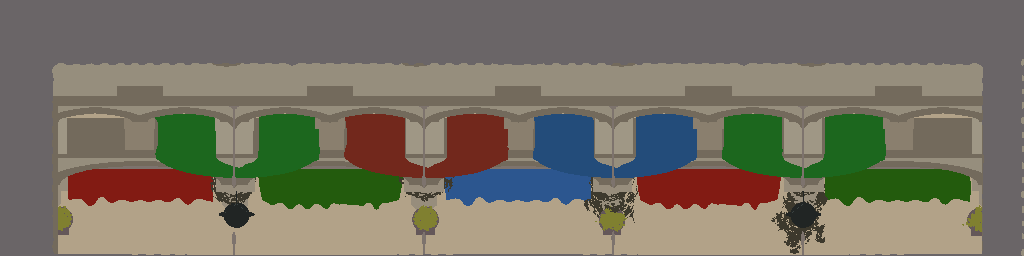
\includegraphics[width=1.0\textwidth]{screenshots/RSM_diffuse}} \\
    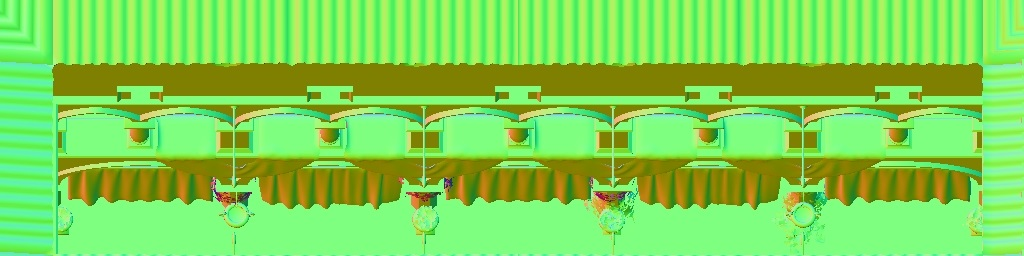
\includegraphics[width=.48\textwidth]{screenshots/RSM_normal} &
    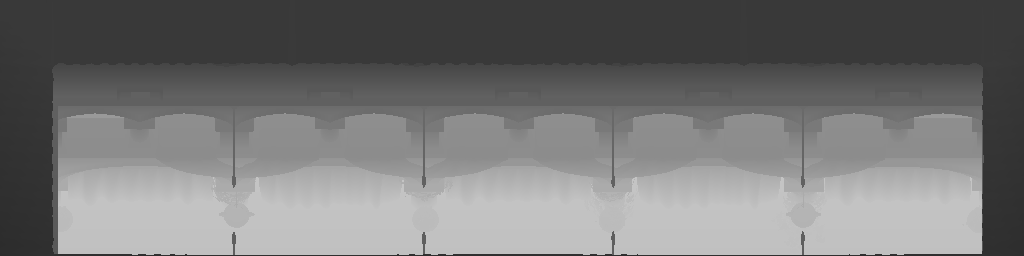
\includegraphics[width=.48\textwidth]{screenshots/RSM_depth}
  \end{tabular}
  \caption{A reflective shadow map, with its diffuse, normal and depth buffer.}
  \label{fig:results:RSMBuffers}
\end{figure}


As explained before, the RSM generation re-uses most of the code of the G-Buffer generation; see \Cref{fig:results:RSMBuffers} for an impression on the rendered result. Accordingly, the performance characteristics are similar to the regular geometry pass of deferred renderers.

Since the implemented VPL sampling distributes the samples over the entire shadow map, we simply limited the VPLs' locations to the relevant area by tuning the light's extents. As a result, an aspect ratio chosen specifically for each test scene is used.

As our implementation re-uses the RSM as shadow map for direct lighting, we chose a resolution of 512\,px² (or, in the case of the Sponza scene, 1024x256\,px), which is more than required by the naive VPL sampling. The RSM is rendered in 0.17\,ms for the Sponza scene.

The VPL sampling itself takes only several microseconds and is negligible. Bear in mind that, in order to achieve high quality levels, a more elaborate sampling algorithms needs to be implemented, which can actually take most of the available time.

\begin{figure}[htb]
\centering
  \begin{tabular}{@{}c@{}}
    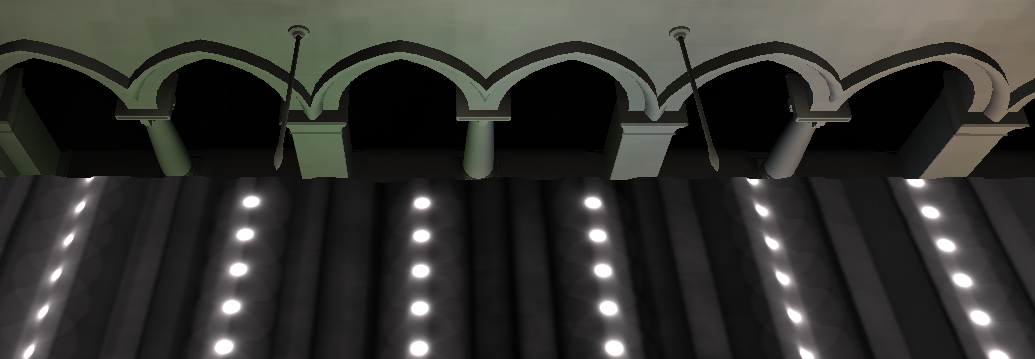
\includegraphics[width=1.0\textwidth]{screenshots/RSM_unfavorable} \\
  \end{tabular}
  \caption{A visualization of inefficiently placed VPLs. Each of the brigth spots is a VPL. Here, they are all placed on the roof pointing upwards. Since there is no further geometry above them that could be illuminated, they do not contribute to the final image.}
  \label{fig:results:RSMUnfavorable}
\end{figure}

The sampling does not take the relevance of the sampled VPLs to the current frame into account and causes the entire system to be rather inefficient by choosing lights that might contribute little or nothing to the rendered output. See \Cref{fig:results:RSMUnfavorable} for an example of unfavorable VPL locations.

An additional downside of the naive sampling is the poor temporal stability when the scene light moves. This is due to each VPL staying at the exact same position in the light's viewport, so they strictly ``follow'' the light's movement, jumping over depth discontinuities along the way. See \Cref{???} for a figure visualizing the frame-to-frame coherency.

\todo{frame-to-frame coherencey screenshots/visualization}


\section{ISM Rendering}

This section presents the results for visibility testing using Imperfect Shadow Maps. The next three subsections will show the outcome in terms of quality, performance and memory usage. The technique does not handle high geometric complexity of the test scenes well; this is detailed in the fourth subsection. Afterwards, the two different ISM renderers are compared and the suitability of ISMs for global illumination in general is discussed.


\subsection{Quality}
\label{sec:results:ism:quality}

\begin{figure}[htb]
\centering
  \begin{tabular}{@{}cc@{}}
    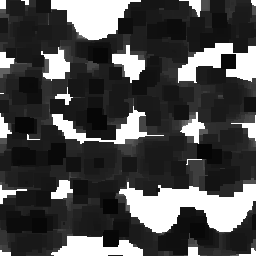
\includegraphics[width=.48\textwidth]{screenshots/ism_splat_cropped} &
    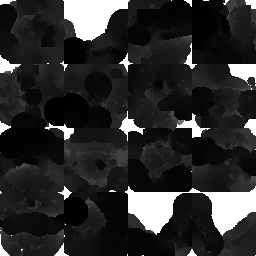
\includegraphics[width=.48\textwidth]{screenshots/ism_single_pixel_cropped}
  \end{tabular}
  \caption{ISMs rendered using the splat renderer (left) and single-pixel renderer (right) with default settings. The single-pixel renderer performs interpolation between points, uses more points and does not let points ``bleed'' into neighboring ISMs, but takes more time.}
  \label{fig:results:isms}
\end{figure}

\Cref{fig:results:isms} shows a few ISMs rendered with the splat and single-pixel renderer. The imperfections do show, and not only through the low resolutions. The distortion of the surface silhouettes by the splat renderer or postprocessing contribute their part, making it hard to identify which part of the Crytek Sponza is shown. However, keep in mind that ???
\todo{???}

\begin{figure}[htb]
\centering
  \begin{tabular}{@{}cc@{}}
    \includegraphics[width=.48\textwidth]{screenshots/darkening_splat} &
    \includegraphics[width=.48\textwidth]{screenshots/darkening_single_pixel}
  \end{tabular}
  \caption{Darkening caused by the splat renderer (left) compared to the single-pixel renderer (right). Note that there is no skylight rendered, which leads to an unnaturally dark upper part in the image even for the single-pixel renderer.}
  \label{fig:results:ismDarkening}
\end{figure}

Comparing the screenshots in \cref{fig:results:ismDarkening}, it becomes apparent that the splat renderer causes visible darkening in the upper part of the image. The reason is likely that the point splats are always oriented towards the camera and do not take the point's normal into account when rendering, amplifying the usual aliasing artifacts of common shadow maps. As a result, any point size larger than one pixel causes surfaces that are not directly facing the camera appear nearer than they actually are when doing shadow lookups in ISMs. A larger shadow bias could compensate for that but would introduce heavier light leaking. Another possibility is to use the normal to calculate a point's depth per fragment at a potentially high performance cost.

As the single-pixel renderer does not use splats, it does not have this problem. In a certain way it performs the per-fragment depth calculation implicitly during interpolation in the postprocessing phase.


\begin{figure}[htb]
\centering
  \begin{tabular}{@{}cc@{}}
    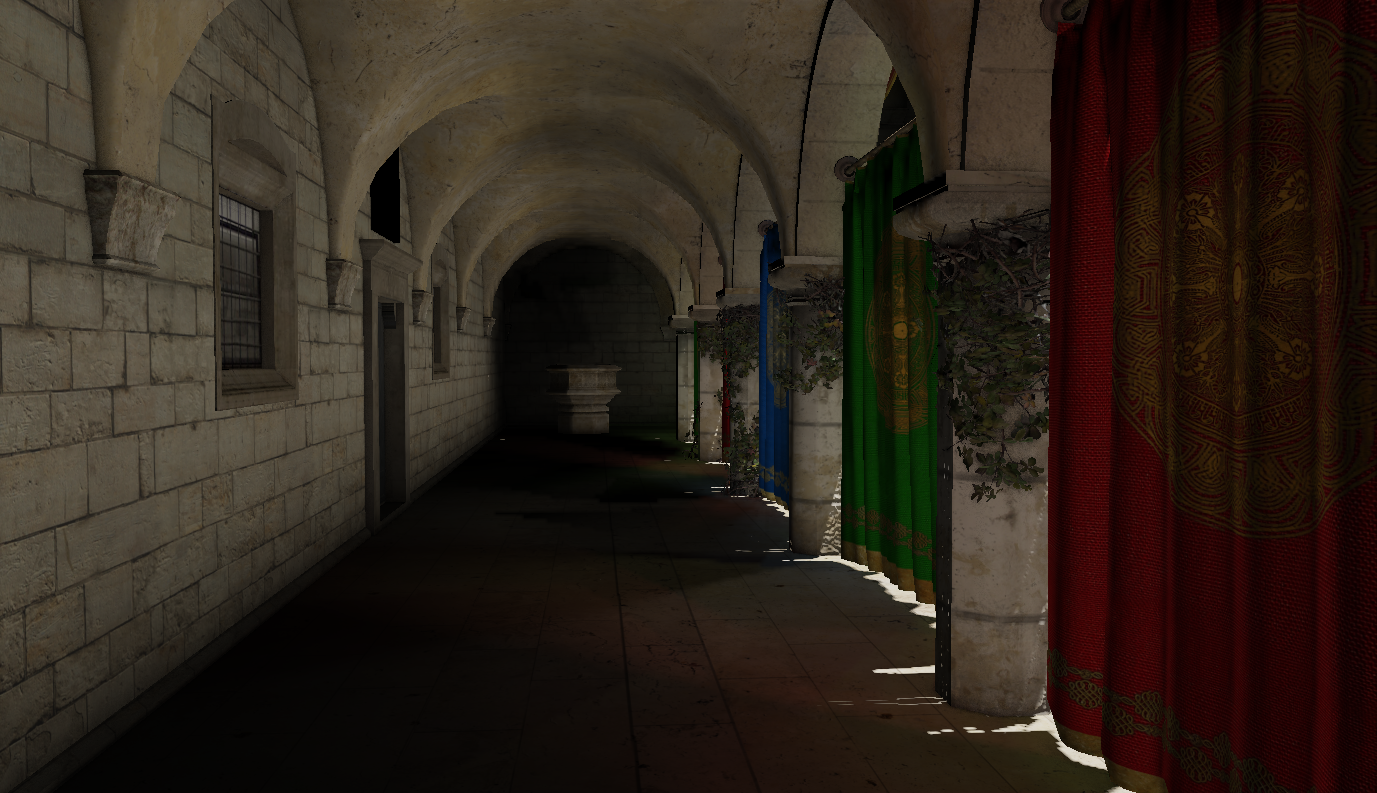
\includegraphics[width=.48\textwidth]{screenshots/leaks_splat} &
    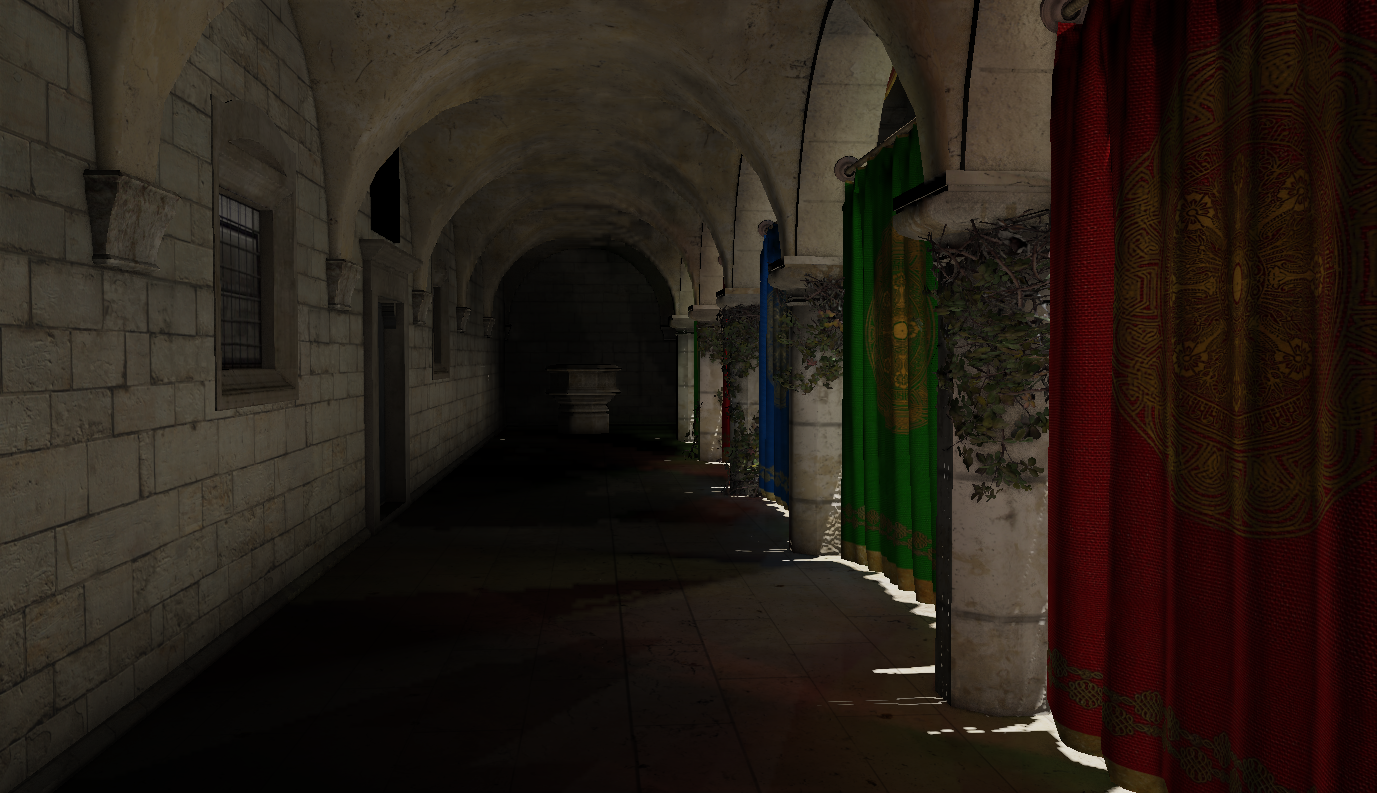
\includegraphics[width=.48\textwidth]{screenshots/leaks_single_pixel}\\
    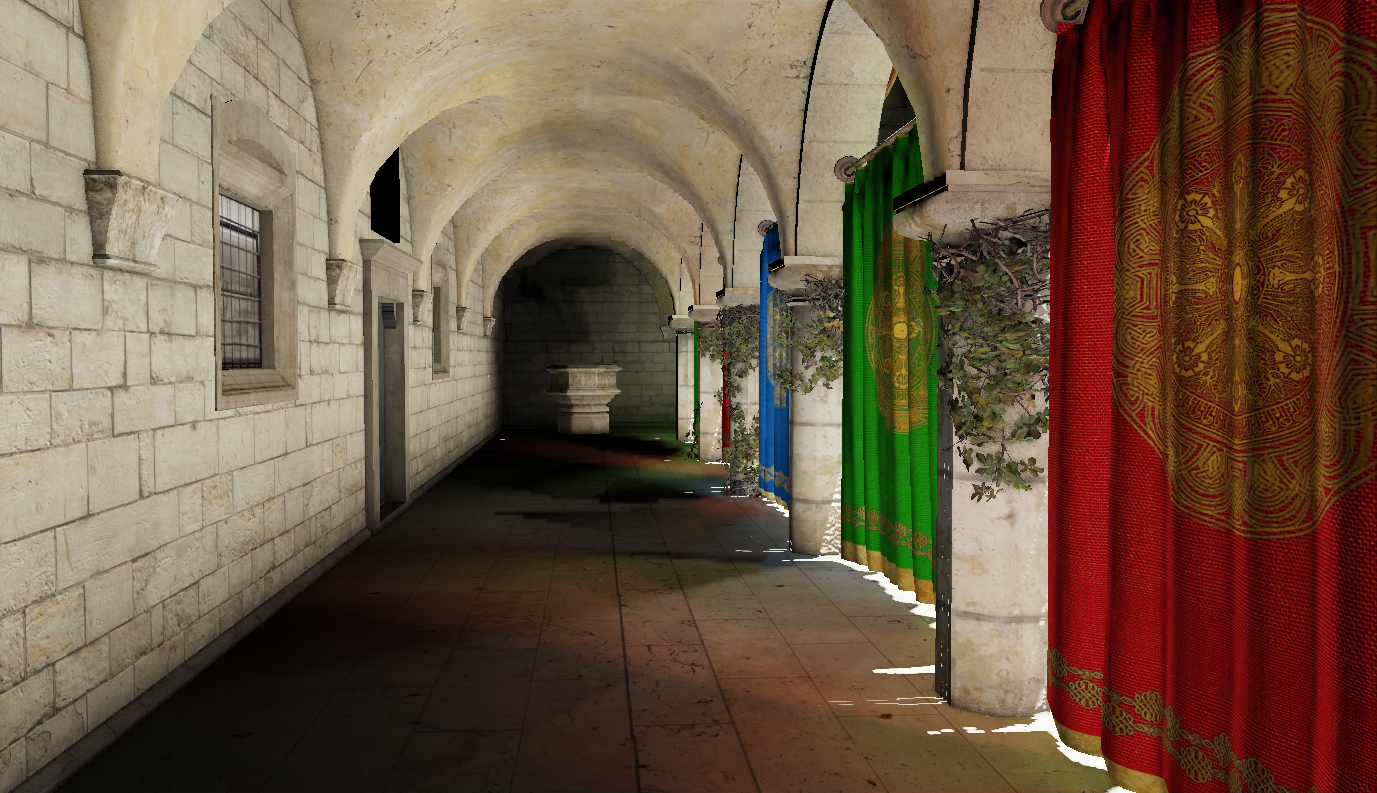
\includegraphics[width=.48\textwidth]{screenshots/leaks_splat_exposure} &
    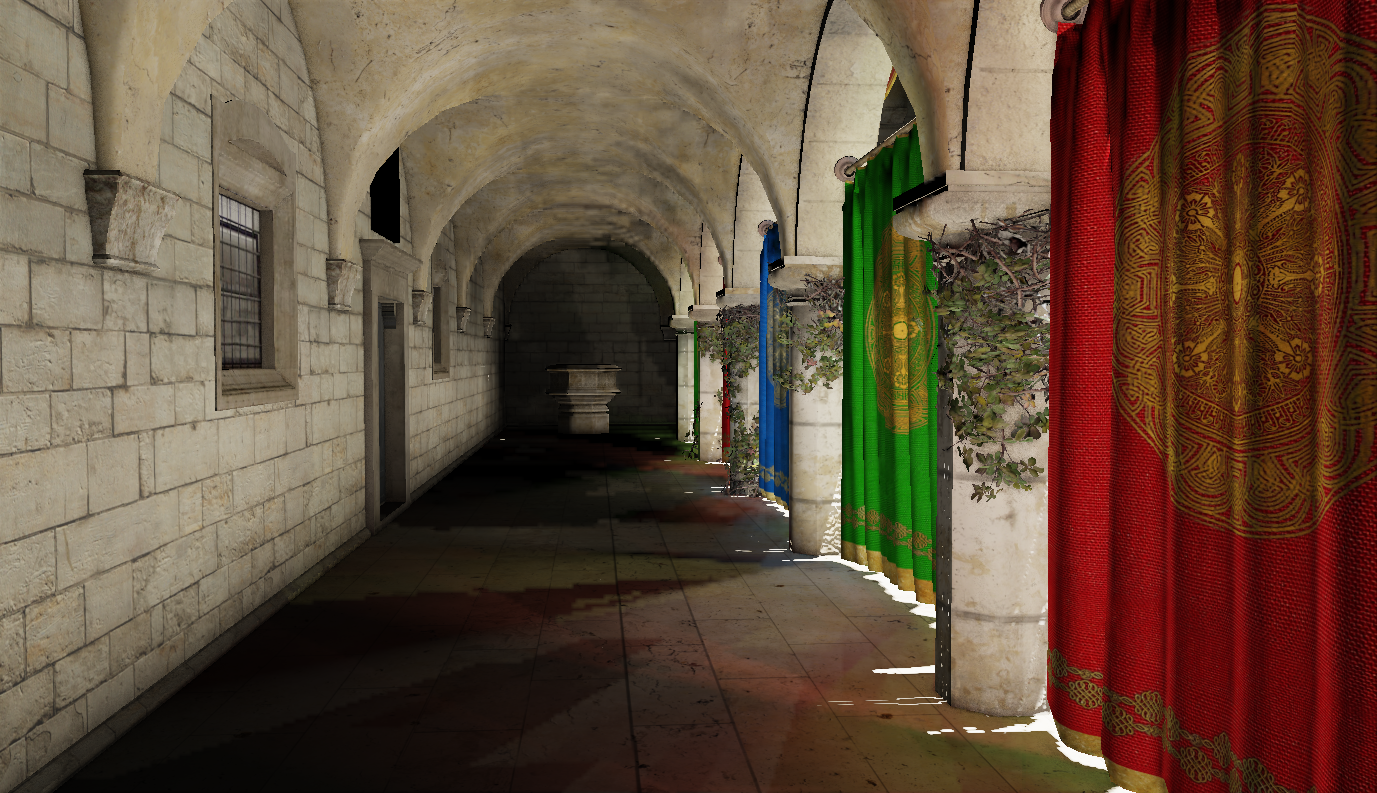
\includegraphics[width=.48\textwidth]{screenshots/leaks_single_pixel_exposure}
  \end{tabular}
  \caption{Light leaks caused by imperfect shadow maps rendered with the splat renderer (left) and single-pixel renderer (right). VPLs from beneath the curtains leak light onto the wall and ceiling, while VPLs on the pillars and curtains light the floor. The renderings in the bottom row use a higher exposure for illustration. }
  \label{fig:results:leaks}
\end{figure}


\Cref{fig:results:leaks} shows a case the ISM technique has difficulties with. The image should be mostly dark or at least uniformly lit through the small gap below the curtains, instead the wall and ceiling receive a lot of light and the floor displays several artifacts. The root cause is that the VPLs are placed right behind the curtains, so the occluding geometry, i.\,e., the curtain, is very near to the light source. Due to the randomness involved when selecting point sets for rendering ISMs, it often happens that the points near to the light source are rendered into other ISMs, leaving a large hole behind. The single-pixel renderer copes a bit better than the splat renderer since it uses more points, but does not provide a satisfactory result either.



\begin{figure}[htb]
\centering
  \begin{tabular}{@{}cc@{}}
    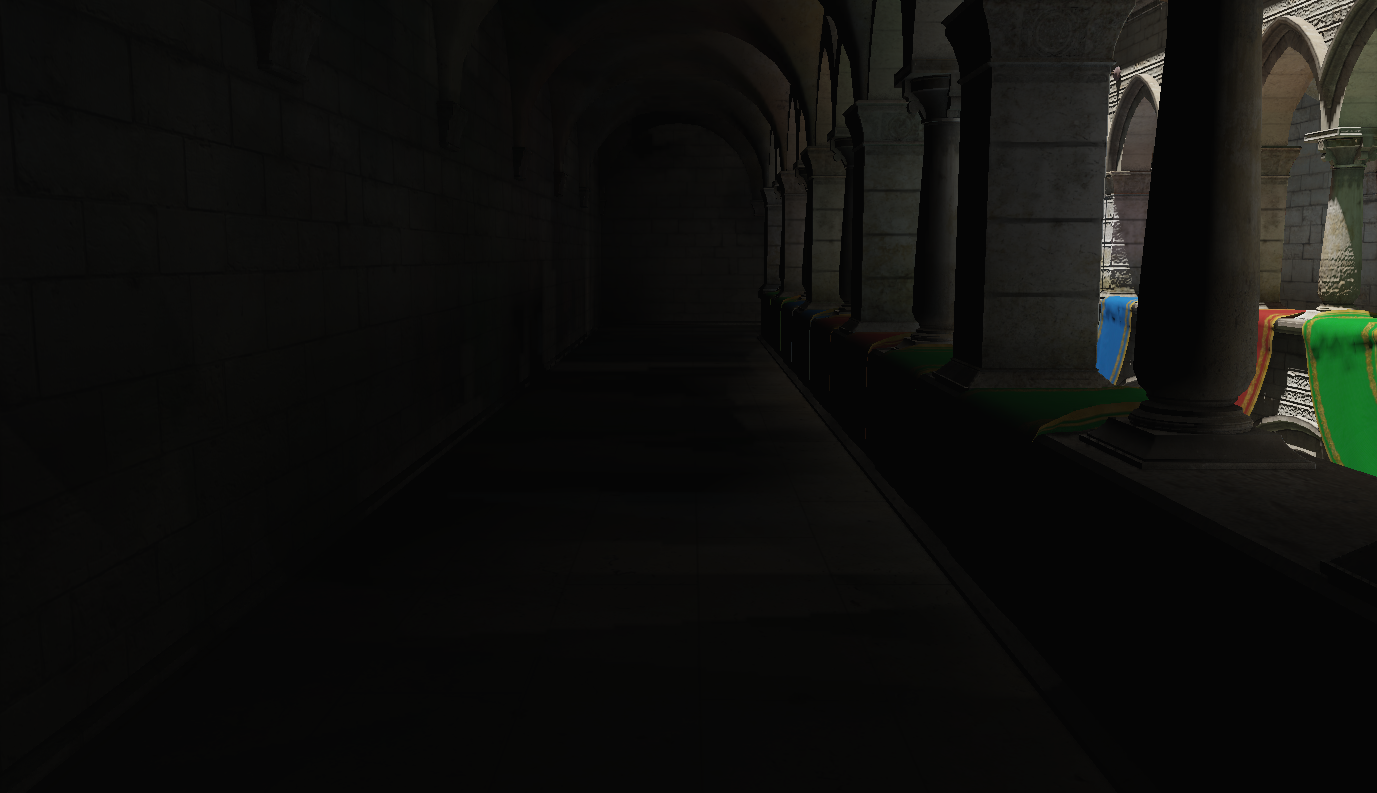
\includegraphics[width=.48\textwidth]{screenshots/bias_splat} &
    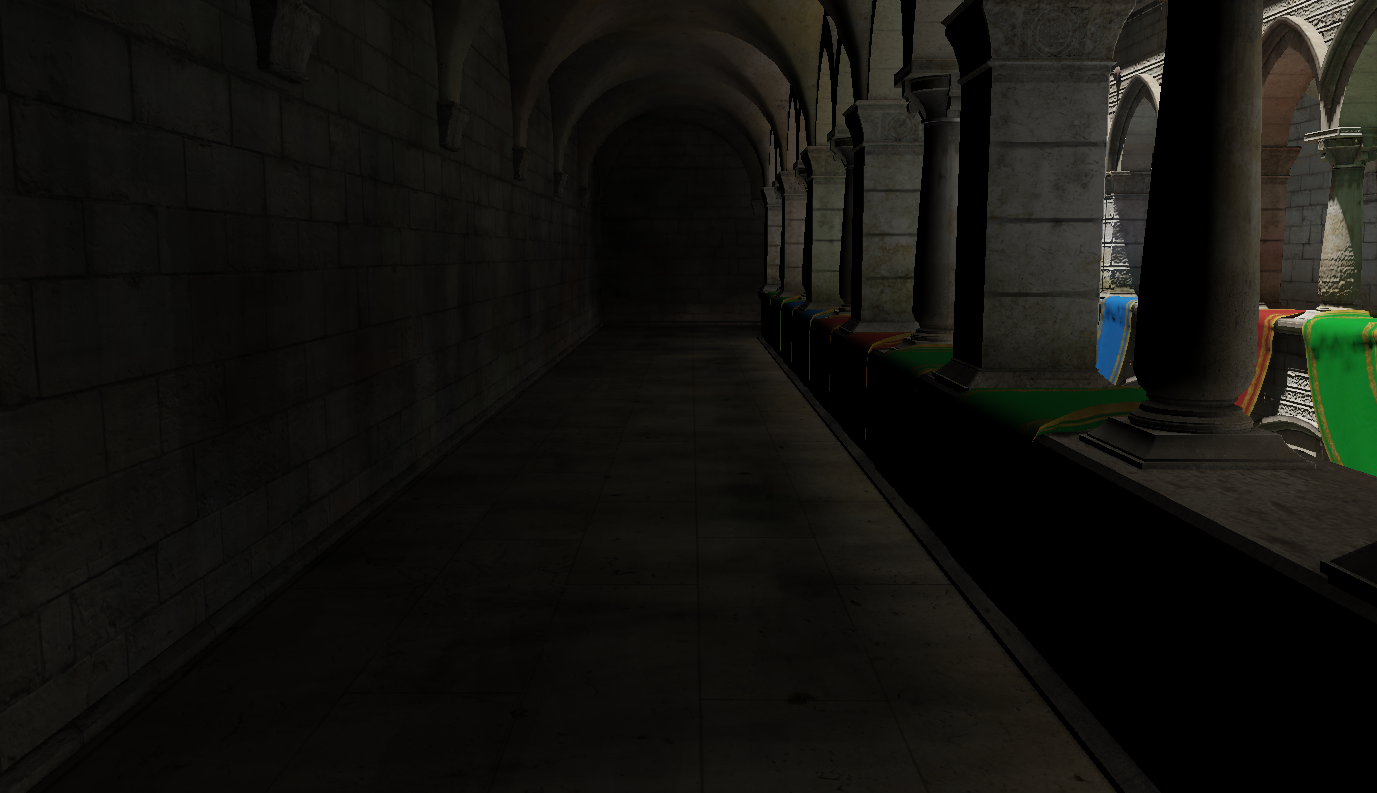
\includegraphics[width=.48\textwidth]{screenshots/bias_single_pixel}\\
      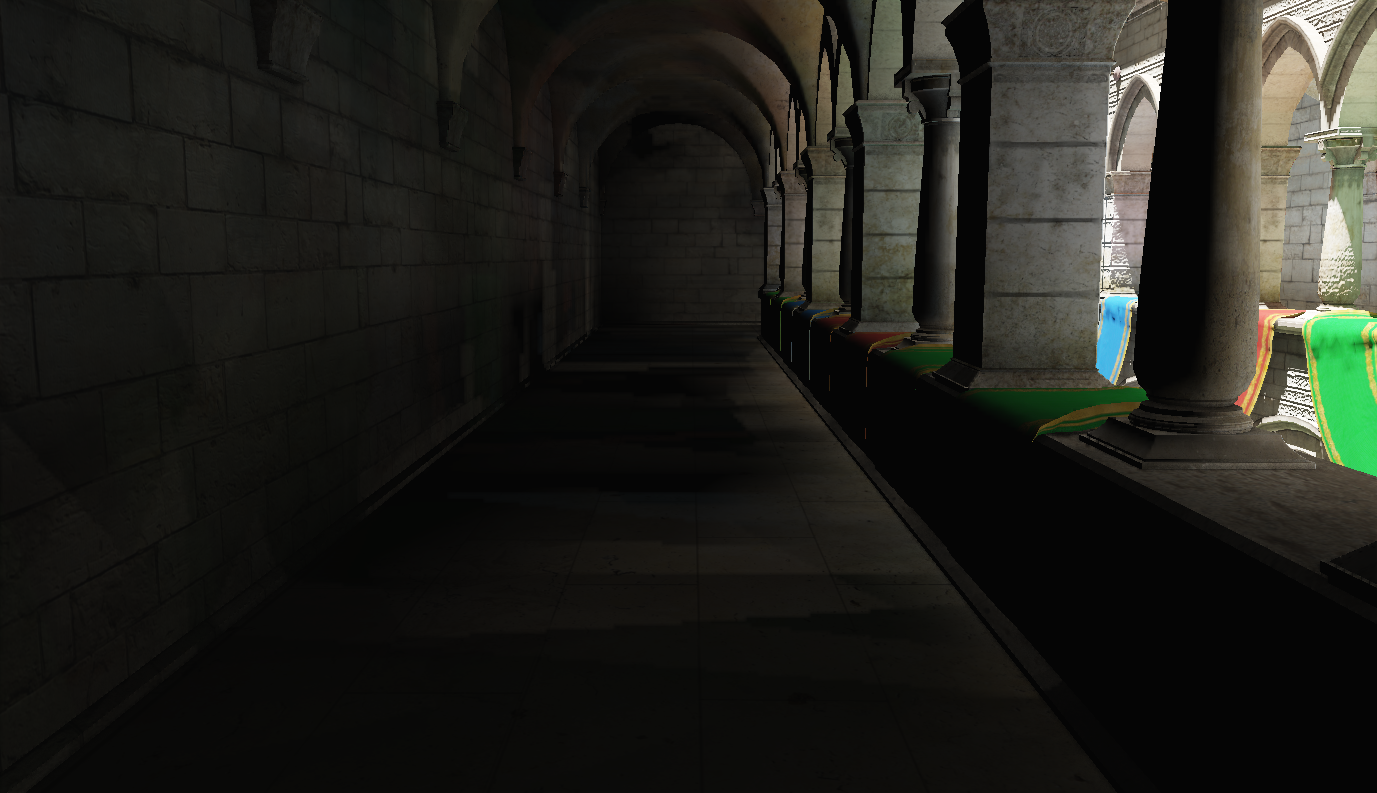
\includegraphics[width=.48\textwidth]{screenshots/bias_splat_exposure} &
      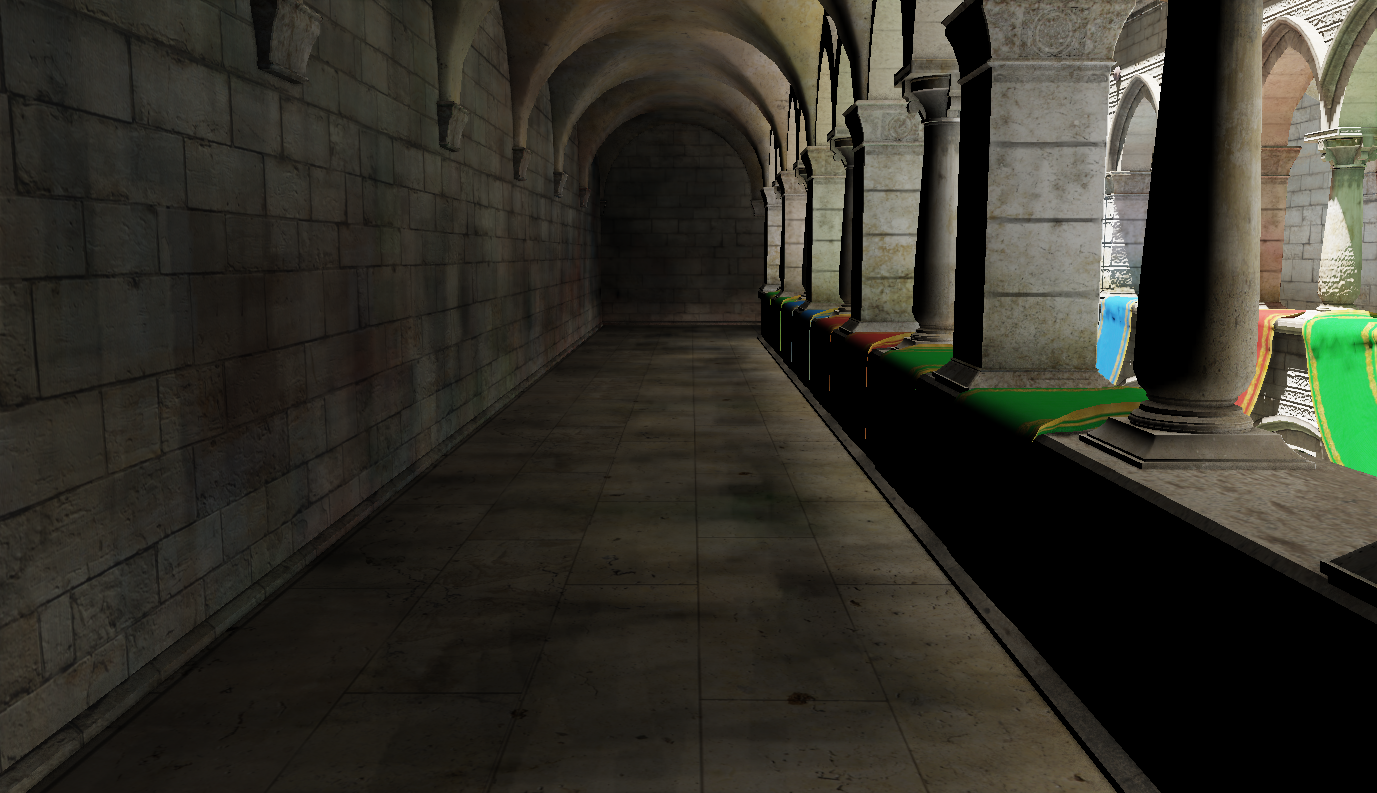
\includegraphics[width=.48\textwidth]{screenshots/bias_single_pixel_exposure}
  \end{tabular}
  \caption{Light leaks caused by using a relatively large shadow bias with the purpose to hide artifacts of the ISMs. The screenshots to the left use the splat renderer, the right ones the single-pixel renderer. Bottom row uses a higher exposure.}
  \label{fig:results:bias}
\end{figure}

Our implementation hides some of the inaccuracies of ISMs by using a relatively large shadow bias. The resulting light leaks are shown in \Cref{fig:results:bias}. While the splat renderer fares better here, it does so mainly by darkening the whole image since it uses rather large points. The single-pixel renderer on the other hand correctly lets light illuminate the left wall through the columns, but shows a rather noisy result.


\todo{Screenshots when enlarging the points / making them smaller. Discuss.}

\todo{Screenshots when doing more points. either by tessellation or by collecting more. Discuss.}

\todo[color=yellow]{count point for splat renderer and output them somehow.}

\todo{Compare to max quality}

\todo[color=yellow]{implement max quality. every point into every ISM. likely render everything once for each ISM. a checkbox: when checked, compute high-quality once and do not change. back to normal when unchecked.}

\todo{for single-pixel-renderer: maybe show one full-size shadow map to show this *can* work}


\subsection{Performance}
\label{sec:results:ism:performance}

\begin{table}[h]
\begin{center}
    \begin{tabulary}{0.98\textwidth}{| L | L | L | L |}
        \hline
        Splat Default Settings & Single-Pixel Default Settings & Splat with Single-Pixel Settings & Single-Pixel with Splat Settings \\ \hline
        1.08\,ms & 2.74\,ms & 10.14\,ms & 2.31\,ms \\
        \hline
    \end{tabulary}
    \caption{Timings of the ISM renderers with different settings.}
    \label{tab:results:ism_timings}
\end{center}
\end{table}

\Cref{tab:results:ism_timings} shows the time needed for rendering the ISMs with both renderers and different settings.

Note that the comparison between the two renderers with default settings is not a fair one, since the single-pixel renderer uses more points and by default clamps each point's extents to its ISM. If the splat renderer is changed to behave similarly, it takes 0.3 additional milliseconds for clamping, and 8.66 additional milliseconds for using the same technique to collect VPLs as the single-pixel renderer does. There are several reasons for this heavy slowdown: First, this is implemented by emitting multiple vertices in the geometry shader, which is known to have poor performance on current GPUs. Second, the additional fillrate and overdraw became an issue when using too many points, a bottleneck that is unlikely to occur when using the single-pixel renderer. And third, while the single-pixel renderer uses shared memory to load the 16 VPLs once, the geometry shader of the splat renderer has no access to shared memory and has to load all 16 VPLs per invocation, creating high register pressure.

Conversely, if the single-pixel renderer does not perform clamping, the push phase needs 0.07\,ms less (0.85\,ms to 0.78\,ms), and when it considers only one VPL per point, the point renderer uses 0.41\,ms less (0.65\,ms to 0.24\,ms).

Since the presented implementation uses no adaptivity, these numbers are independent from the viewport. They are however slightly affected by VPL placement, since it influences culling. In a second scenario, where the sunlight shines directly from above, all VPLs are placed on the floor facing up. As a result, much fewer points are culled during ISM rendering, resulting in slightly higher timings. Both renderers need about 0.1\,ms more in this case.

\todo{Numbers when enlarging the points / making them smaller. Discuss. Note how the single-pixel renderer is (hopefully) not affected by point size.}

\todo{Numbers when doing more points. either by tessellation or by collecting more. Discuss.}


\subsubsection{Detailed Performance Measurements for the Single-Pixel Point Renderer}
\label{sec:results:ism:performanceSinglePixelRenderer}


\begin{table}[h]
\begin{center}
    \begin{tabulary}{0.98\textwidth}{| L | L | L | L || L |}
        \hline
        Point Collection & Point Rendering & Pull Phase & Push Phase & Total\\ \hline
        0.83\,ms & 0.65\,ms & 0.39\,ms & 0.85\,ms & 2.72\,ms\\
        \hline
    \end{tabulary}
    \caption{Timing breakdown of the single-pixel point renderer.}
    \label{tab:results:timing_breakdown_single_pixel}
\end{center}
\end{table}

\begin{table}[h]
\begin{center}
    \begin{tabulary}{0.98\textwidth}{| L | L | L | L | L | L | L | L || L | L || L |}
        \hline
        PL 1 & PL 2 & PL 3 & PL > 3 & PS > 2 & PS 2 & PS 1 & PS 0 & PL Total & PS Total & Total \\ \hline
        0.16 & 0.16 & 0.04 & 0.03   & 0.06   & 0.08 & 0.30 & 0.41 & 0.39     & 0.85     & 1.24\\
        \hline
    \end{tabulary}
    \caption{Timing breakdown of the pull (PL) and push (PS) phase. The numbers of the individual steps indicate to which mipmap level they write, which is why the pull phase starts with 1 and the push phase has descending numbers. All timings are in milliseconds.}
    \label{tab:results:timing_breakdown_pull_push}
\end{center}
\end{table}


\Cref{tab:results:timing_breakdown_single_pixel} gives more detailed performance measurements of the single-pixel renderer, while \cref{tab:results:timing_breakdown_pull_push} further breaks down the individual steps of the pull and push phase. Note how the timings scale roughly as expected (PL 3 and PS 2 are taking roughly 4 times longer than PL 2 and PS 1, respectively), but not so the first and last step. This is due to the reduced input data size (or output size, respectively), as explained in \cref{sec:impl:pullPushPostprocessing}. Also note how the push phase does take roughly the time of the pull phase if it were not for the last phase, where it writes to the full 2048\,px² of miplevel zero, whereas the largest miplevel written to by the pull phase is level one with 1024\,px².

\todo{Impact of packing?}


\subsection{Memory Usage}
\label{sec:results:ism:memory}

The point splat renderer uses no more memory than the ISM texture itself requires, which is 8\,MB for a 2048\,px² 16-bit depth buffer.

The single-pixel renderer uses additional memory. First, it uses a buffer for storing the points. This is implemented as four-channel 32-bit float texture, with the first three channels containing the position, and the last channel containing radius (8 bit) and normal (24 bit, see \cite{Cigolle:2014:NormalPacking}). With a maximum point count of 2048 per ISM (keep in mind they are rendered into multiple ISMs later), this buffer uses 32\,MB.
The additional textures used are the render target of the single-pixel renderer (single-channel 2048x2048\,px, 32-bit integer, uses 16\,MB), the mipmap levels used by the pull-push algorithm (four channels, 32-bit, use approx. 22\,MB) and the final ISM (same format as used by the splat renderer, uses 8MB).

Added together, the single-pixel renderer uses a total of 79\,MB. There is some room for optimization left: For instance, one channel of the mipmap levels is unused (OpenGL does not offer three-channel images), and in some places, using 16-bit floats instead of 32-bit float might be sufficient.


\subsection{Problems with High Geometric Density}
\label{sec:results:ism:densityProblems}

As a more demanding test case is the San Miguel scene with 7.9M triangles. The most apparent problem of the presented implementation is the lack of adaptivity to the current viewport in addition to the lack of LOD methods. As a result, all 7.9M triangles are used every frame to render the ISMs, with corresponding performance results: The point collection phase of the single-pixel renderer now takes 12.0\,ms, while the point rendering uses an additional 5.3\,ms. The time needed by the postprocessing is unchanged since it works on fixed resolution textures. The splat renderer uses 12.0\,ms, which is the exact same amount of time as the point collection phase of the single-pixel renderer, even though the latter does no rasterization work. This demonstrates how this process is bottlenecked by geometric complexity.


\begin{figure}[htb]
\centering
  \begin{tabular}{@{}c@{}}
    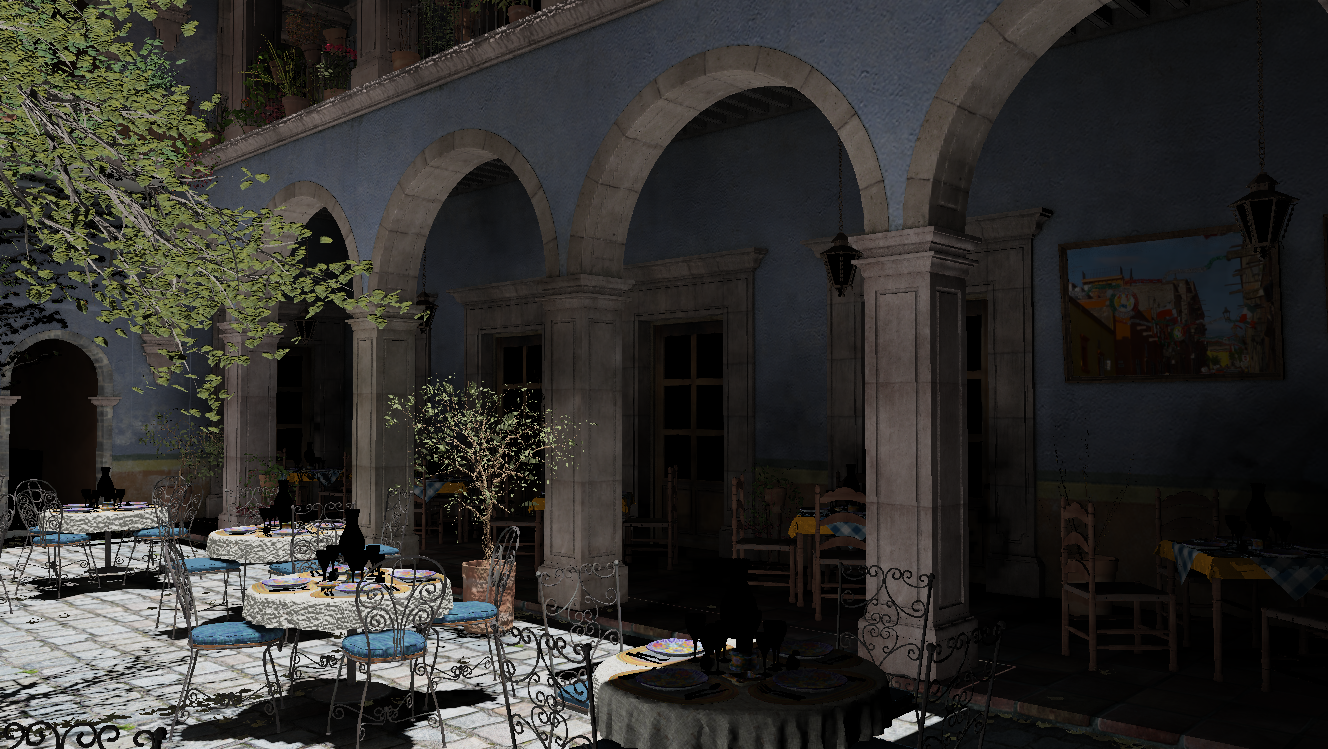
\includegraphics[width=1.0\textwidth]{screenshots/san_miguel_wide} \\
  \end{tabular}
  \caption{A rendering of the San Miguel scene in the presented implementation. Note the unnaturally dark region behind the pillars.}
  \label{fig:results:san_miguel_wide}
\end{figure}

\begin{figure}[htb]
\centering
  \begin{tabular}{@{}cc@{}}
    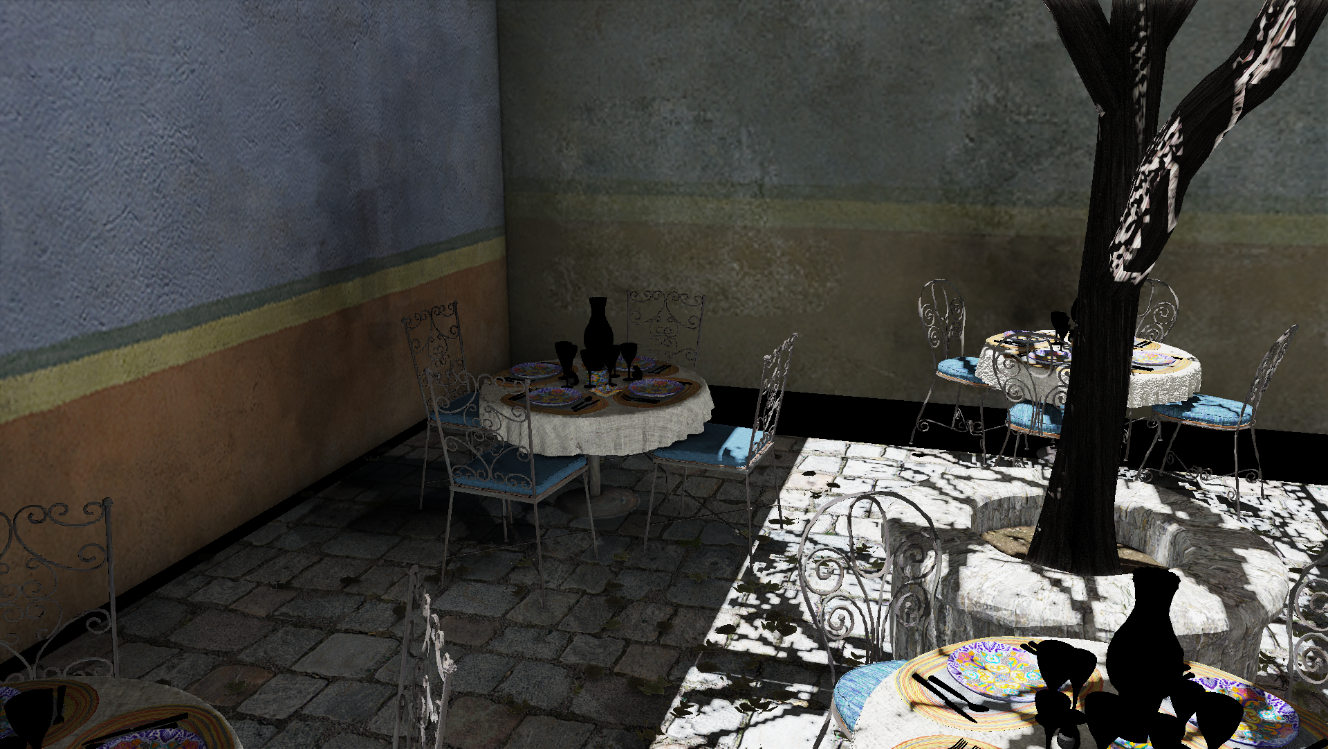
\includegraphics[width=.48\textwidth]{screenshots/san_miguel_ugly_shadow} &
    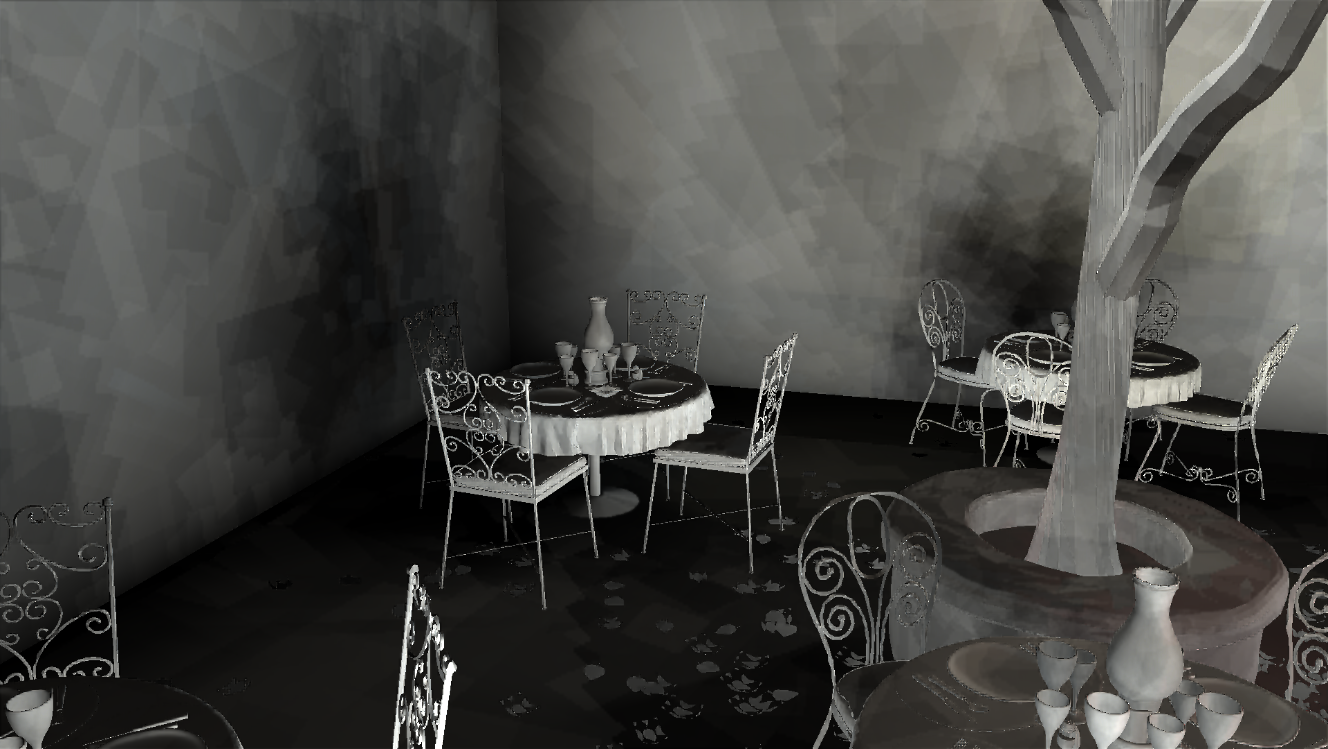
\includegraphics[width=.48\textwidth]{screenshots/san_miguel_ugly_shadow_gi_only}
  \end{tabular}
  \caption{A particularly inaccurate shadow produced by ISMs. Right image shows only indirect light. Ideally, the shadow would be much more smooth. The low-frequency noise is caused by choosing random points per ISM, while the many edges of the shadows are caused by the basic shadow mapping algorithm, which performs a simple binary choice.}
  \label{fig:results:san_miguel_ugly_shadow}
\end{figure}

\Cref{fig:results:san_miguel_wide} shows an example screenshot of the San Miguel scene. There are several factors contributing to an overly dark region behind the pillars. First, during ISM rendering all points are rendered into at least one pixel, making them take out too much light if they are actually smaller than one pixel. This likely happens in case of the thin structures of the chairs and trees. Additionally, the implementation simulates only one bounce, making it impossible for the floor behind the pillars to be lit at all.

Another problem case is shown by \Cref{fig:results:san_miguel_ugly_shadow}, where the table and chairs cast a visibly inaccurate shadow.


\subsection{Comparison of the Splat and Single-Pixel Renderer}
\label{sec:results:ism:comparison}

The single-pixel renderer provides numerous advantages over the splat renderer: Using a compute shader to render points lifts the restrictions of the fixed-function pipeline and, e.\,g., enables rendering each point into multiple ISMs without large performance losses. Quality-wise, it can reproduce surfaces more accurately by correctly interpolating between points.

The drawbacks obviously include the additional rendering time and memory. Besides, the added complexity should not be underestimated. Specifically, we found it hard to fine-tune the pull-push algorithm to produce satisfactory results, especially in the face of the low resolutions of ISMs and the limited data available for reconstruction after selecting a random and sparse set of points.

\todo{Add notes about scaling when i have point counts}



\subsection{Discussion}
\label{sec:results:ism:discussion}

Imperfect shadow maps have several deficits, some of which are inherent to the technique and difficult to solve, others are specific to the implementation choices and tradeoffs in the presented implementation and might be easier to overcome.

First, ISMs reduce the scene's geometry to points. At the resolution that is achievable in a real-time budget, this is already a rough approximation that loses a lot of accuracy.

Second, because a sparse set of points is used for each ISM, each point must be enlarged to accommodate for the neighboring points that are likely missing in the chosen ISM. For instance, if an area is represented by a thousand points and only one tenth of all points is used for each ISM, each remaining point's area must be enlarged by a factor of ten to result in an equally large area in the rendered output. Of course, this approach leads to deformed geometry since points at the edges of the area get enlarged as well, growing over the borders of the original geometry.

Third, ISMs also have numerical issues. For instance, both the splatting and postprocessing approaches ignore the distortion caused by the paraboloid projection, and thus might render even simple surfaces incorrectly. This contributes to the necessity of using a relatively large shadow bias. At the cost of additional complexity, this can likely be solved.

Fourth, and this is in our view the most important shortcoming, ISMs handle geometry in the vicinity to VPLs badly as can be seen in \cref{fig:results:leaks}. To sufficiently approximate such surfaces when rendering ISMs, one would need to greatly increase the number of points created near VPLs, possibly in addition to stepping away from using a fully random approach for point selection and select a specific point set for each ISM depending on the VPLs location.

As for most global illumination algorithms, a massive improvement would be to differentiate between large-scale scene geometry that is important for diffuse light bounces, and smaller geometry of lesser importance. While the latter can possibly be ignored altogether with only minor losses in quality, the shape of large-scale geometry is all the more important to preserve (relatively) precisely.

The San Miguel scene is a good example for this: While the small detail work like dishes and small plants make up most of the geometry and thus most of the rendering time, they contribute only very little to global illumination. This is where the presented implementation suffers most from the lack of level-of-detail methods.


\todo[color=yellow]{implement some moving object. show temporal coherency when it moves. or even moving spherical light.}


\section{Interleaved Shading with Compute Shaders}
\label{sec:results:interleavedShading}

Interleaved shading substantially reduces the number of lights that are processed per pixel. Using a 4x4 interleaving pattern, each pixel processes only a sixteenth of all lights, ideally speeding up the final gathering phase by a factor of 16. However, an additional blur pass is required to mask the noise that results from interleaving, which takes additional time.


\begin{table}[h]
    \begin{center}
        \begin{tabulary}{0.98\textwidth}{| L | L | L | L | L |}
            \hline
            Without IS & With IS & Speedup & Blur Pass & Speedup with Blur\\ \hline
            40.24\,ms & 2.61\,ms & 15.42 & 0.63\,ms & 12.42\\
            \hline
        \end{tabulary}
        \caption{Timings of interleaved shading (IS) with a block size of 4x4. Note that the blur pass is mandatory when using interleaved shading; the middle column merely illustrates the efficiency of the presented implementation, while the last column shows the practical speedup that is achieved.}
        \label{tab:results:timings_interleaved_shading}
    \end{center}
\end{table}



\begin{figure}[htb]
    \centering
    \begin{subfigure}[b]{0.20\textwidth}
        \centering
        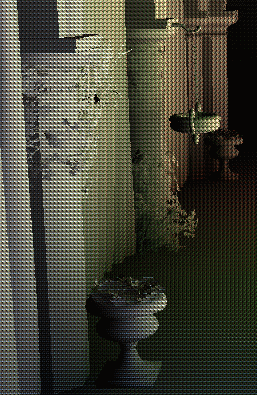
\includegraphics[width=.95\textwidth]{screenshots/interleaved_before}
        \caption{}
        \label{fig:results:interleaved_before}
    \end{subfigure}%
    \begin{subfigure}[b]{0.20\textwidth}
        \centering
        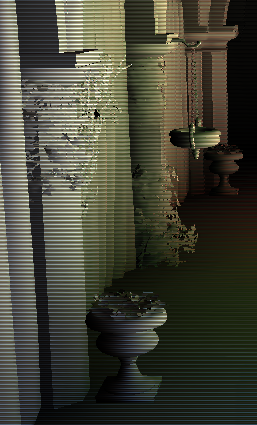
\includegraphics[width=.95\textwidth]{screenshots/interleaved_horizontal_blur}
        \caption{}
        \label{fig:results:interleaved_horizontal_blur}
    \end{subfigure}%
    \begin{subfigure}[b]{0.20\textwidth}
        \centering
        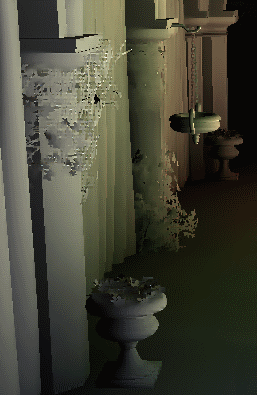
\includegraphics[width=.95\textwidth]{screenshots/interleaved_final}
        \caption{}
        \label{fig:results:interleaved_final}
    \end{subfigure}%
    \begin{subfigure}[b]{0.20\textwidth}
        \centering
        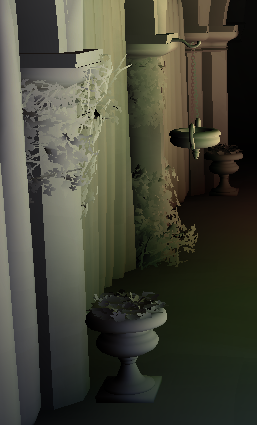
\includegraphics[width=.95\textwidth]{screenshots/interleaved_without}
        \caption{}
        \label{fig:results:interleaved_without}
    \end{subfigure}%
    \begin{subfigure}[b]{0.20\textwidth}
        \centering
        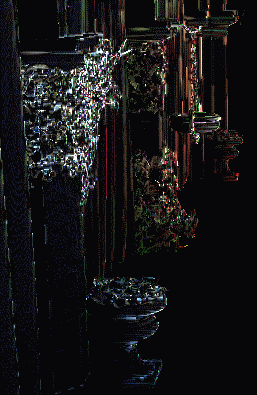
\includegraphics[width=.95\textwidth]{screenshots/interleaved_difference_gi}
        \caption{}
        \label{fig:results:interleaved_difference_gi}
    \end{subfigure}
    \begin{subfigure}[b]{0.32\textwidth}
        \centering
        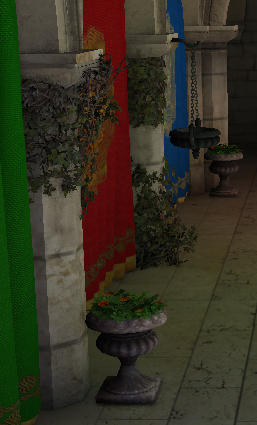
\includegraphics[width=.95\textwidth]{screenshots/interleaved_without_textured}
        \caption{}
        \label{fig:results:interleaved_without_textured}
    \end{subfigure}
    \begin{subfigure}[b]{0.32\textwidth}
        \centering
        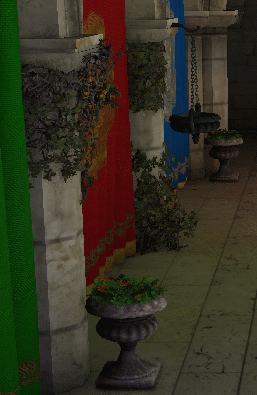
\includegraphics[width=.95\textwidth]{screenshots/interleaved_with_textured}
        \caption{}
        \label{fig:results:interleaved_with_textured}
    \end{subfigure}
    \begin{subfigure}[b]{0.32\textwidth}
        \centering
        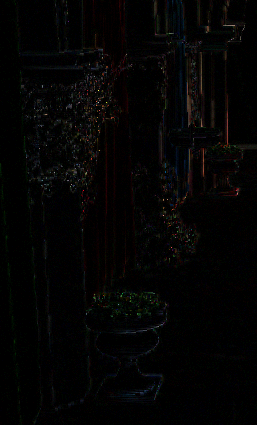
\includegraphics[width=.95\textwidth]{screenshots/interleaved_difference_shaded}
        \caption{}
        \label{fig:results:interleaved_difference_shaded}
    \end{subfigure}

      \caption{Interleaved shading results. Top row shows indirect light only. From left to right: (a) Result of the final gathering phase without the geometry-aware blur, (b) with the horizontal phase of the blur applied, (c) with both phases applied, (d) result of the final gathering phase without using interleaved shading, (e) difference between (c) and (d). Bottom row: (f) final result after blending when using interleaved shading, (g) whithout interleaved shading, (h) difference between (f) and (g). Difference values are multiplied by four.}
      \label{fig:results:interleaved_quality}
\end{figure}


\Cref{tab:results:timings_interleaved_shading} shows timings of the presented implementation. Most notably, the interleaved shading technique introduces very little overhead, as indicated by the speedup of 15.42 compared to the theoretical maximum of 16. In absolute terms, a speedup of 16 would require the final gathering phase to take 2.51\,ms. As a result, the technique introduces 0.1\,ms of overhead.

When considering the blur phase, the overhead adds up to 0.73\,ms and the speedup is lowered to 12.42. Of course this is still a substantial improvement, especially considering the negligible quality impact.

This technique uses an additional buffer for storing the intermediate result of the blur phase, while the final result can be written into the same texture that was used for final gathering. The texture format \texttt{GL\_R11F\_G11F\_B10F} is used here, resulting in roughly 2\,MB additional storage at full HD. The presented implementation does not re-use the final gathering texture to keep the results of all stages available for debugging purposes.


\subsubsection{Discussion}
Interleaved shading is an obvious win for many-light global illumination methods. Paying the full cost of evaluating all VPLs per shading point is simply unnecessary due to the low-frequency nature of global illumination. Adapting the shading frequency to a similarly low level is the only reasonable choice for real-time applications.

In fact, given the unnoticable quality impact (\Cref{fig:results:interleaved_quality}) of interleaved shading when using a 4x4 block size, larger block sizes, e.\,g., 8x8 as used by \citet{hedman2016sequential} should be considered. Especially with the advent of high-resolution displays, lowering the shading frequency of global illumination effect even further might be necessary to keep the costs down to a reasonable level. However, the performance gains from lower sample counts will be offset in part by larger blur radii that come with larger block sizes.

Going further, this technique is limited by how well the blur phase will be able to mask the noise in more difficult areas with lots of depth discontinuities like vegetation. It seems imaginable to extend interleaved shading with ???, which collect fragments that receive too few information during shading with the purpose to perform a second pass on those fragments, enhancing the problematic areas. Temporal reprojection methods that re-use information from previous frames and use different sets of VPLs per frame would be another natural extension of interleaved shading.

\todo{that fragment collecting reference}

\todo{put VPL shuffling comparison anywhere}



\section{Clustered Deferred Shading}
\label{sec:results:clusteredShading}

Clustered Deferred Shading and Tiled Deferred Shading reduce the number of light calculation operations by clustering fragments and culling lights against those clusters. As such, if implemented correctly, they do not affect quality at all, but are purely performance optimizations.

\begin{table}[h]
    \begin{center}
        \begin{tabulary}{0.98\textwidth}{| L | L | L | L | L |}
            \hline
            Scene & Without CS/TS & With CS & With TS \\ \hline
            Sponza 1 & 3.41\,ms & 2.80\,ms & 2.40\\
            Sponza 2 & 3.94\,ms & 3.63\,ms & 3.09\\
            Sponza 3 & 2.68\,ms & 1.64\,ms & 1.34\\
            San Miguel & 4.75\,ms & 5.21\,ms & 4.43\\
            \hline
        \end{tabulary}
        \caption{Timings of the final gathering stage without optimizations, with clustered shading (CS) and with tiled shading (TS). Each line is a different camera position. Note that the timing ``With CS'' includes roughly 0.06\,ms for the clustering phase and 0.13\,ms for the light list phase.}
        \label{tab:results:timings_clustered_shading}
    \end{center}
\end{table}

As visible in \Cref{tab:results:timings_clustered_shading}, both clustered shading and tiled deferred shading can improve the performance of the final gathering phase considerably, in one of the measurements 50\,\% of the computation time is saved with tiled shading.


It is interesting that clustered shading, being the successor of tiled shading, performs noticeably worse in the context of many-light methods. This is true even for the San Miguel scene, in which the higher amount of depth discontinuities should be favorable to clustered shading. While these performance characteristics might be specific to the presented implementation, there are plausible reasons that they might apply generally: Due to the infinite light radii used, the percentage of culled lights is generally low. Therefore it might be the better choice to optimize for the worst case and implement a low overhead solution like tiled shading, instead of a more accurate solution like clustered shading that might improve the culling rate, but comes with more overhead.

An impression of the amount of overhead introduced by clustered shading is given by the San Miguel scene, from which the last line of measurements is taken. This scene runs much slower even when only considering the final gathering phase, because most VPLs are placed on the walls and floor, pointing inwards or upwards respectively. Therefore much of the geometry lies on the illuminated side of most VPLs, resulting in very little performance gains from culling.

With a low culling rate, clustered shading actually slows down the final gathering phase by 0.46\,ms. While 0.19\,ms of these are fixed costs added by the clustering and light list calculation phases, the final gathering shader itself got 0.27\,ms slower as well. This might be caused by the indirection when accessing lights, since instead of reading from the light buffer directly, the light list with indices is accessed first before reading the light buffer with a dynamic index. Another explanation might be the divergent data flow, since threads from the same work group can access different light lists and thus different light data and shadow maps, possibly hurting cache efficiency.

As discussed in section \Cref{sec:impl:clusteredShading}, clustered shading consumes about 2\,MB of memory. The tiled shading algorithm however, being integrated into the final gathering shader, uses no additional VRAM at all.

\subsubsection{Discussion}

The presented measurements make tiled shading seem like a clear winner, but as so often the situation is more complicated. The integration of tiled shading into the final gathering shader, while an efficient and easy to implement solution, is inherently less flexible than clustered shading. For instance, \citet{olsson2012clustered} propose to use normals as another dimension besides the three spatial ones, further improving culling efficiency. While this is likely easy to integrate into the more flexible approach taken with clustered shading, the integrated tiled shading is constrained by the amount of available shared memory, which makes it challenging to take additional dimensions into account.
